%%%%%%%%%%%%%%%%%%%%%%%%%%%%%%%%%%%
%%%  Filename: main_en.tex
%%%  ---
%%%  Template for Master Thesis at DTETI UGM
%%%  Created using thesisdtetiugm.cls
%%%  --- 
%%%  Written by Canggih Puspo Wibowo
%%%  [canggihpw@gmail.com]
%%%%%%%%%%%%%%%%%%%%%%%%%%%%%%%%%%%

%% Use option "bahasa" or "english" 
%%    to change the basic language used
%% User option "bachelor", "master", or "doctoral"
%% 	  to change the degree

%% TODO: \usepackage graphicx for relative path shortcut
%\documentclass[<bachelor/master/doctoral>,<bahasa/english>]{thesisdtetiugm} 
\documentclass[master,english,table,xcdraw]{thesisdtetiugm} % <table> and <xcdraw> for coloring table

%======================================
% Choose what to be compiled
%   - Comment unedited chapter for fast review compilation
%======================================
\includeonly{
    contents/chapter-1/chapter-1,
    contents/chapter-2/chapter-2,
    contents/chapter-3/chapter-3,
    contents/chapter-4/chapter-4,
    contents/chapter-5/chapter-5
    }
%======================================

%======================================
% Information Input
%======================================
% Input author's name and ID number
\author{<<AUTHOR>>}{<<NIM>>}

% Input the thesis' title
\title{<<Thesis title>>}

% Program and the head of the program
\program{<<Program name>>}{<<Program coordinator>>}{<<NIP>>}
% \program{Master Program Electrical Engineering}{M. Isnaeni Bambang Setyonegoro, Dr. Ir., M.T.}{196510041993031003}

% Name of department head and NIP
\departmenthead{<<Head of the department>>}{<<NIP>>}
\major{<<Major>>}
\yearsubmit{<<year submit>>}
\examdate{<<Exam date>>}
% \departmenthead{Hanung Adi Nugroho, Ir., S.T., M.E., Ph.D., IPM.}{197802242002121001}
% \major{Electrical Power System Concentration}
% \yearsubmit{2023}
% \examdate{\ldots\ldots\ldots}

% Name of thesis supervisors/promotors
\addsupervisor{<<Supervisor 1>>}{<<NIP>>}
\addsupervisor{<<Supervisor 2>>}{<<NIP>>}
\addsupervisor{<<Supervisor 3>>}{<<NIP>>}
% Name of examiners
\addexaminer{<<Examiner 1>>}{<<NIP 1>>}
\addexaminer{<<Examiner 2>>}{<<NIP 2>>}
\addexaminer{<<Examiner 3>>}{<<NIP 3>>}
\addexaminer{<<Examiner 4>>}{<<NIP 4>>}
\addexaminer{<<Examiner 5>>}{<<NIP 5>>}
\addexaminer{<<Examiner 6>>}{<<NIP 6>>}
\addexaminer{<<Examiner 7>>}{<<NIP 7>>}
\addexaminer{<<Examiner 8>>}{<<NIP 8>>}
\addexaminer{<<Examiner 9>>}{<<NIP 9>>}

%======================================
% Initialize nomenclature (!WIP)
%======================================
% \makenomenclature % !WIP
%======================================

%======================================
% Correct bad hyphenation if needed
%======================================
% example correcting bad hyphenation (uncomment to use):
% \babelhyphenation[<<english/bahasa>>]{op-tical net-works semi-conduc-tor}

\begin{document}
%======================================
% Create cover etc
%======================================

%---- PROOF OF SUBMISSIONS ---- 
% \includepdf[pages=-]{private/BUKTI_PENDAFTARAN_PENDADARAN.pdf}

%---- COVER ---- 
% Choose one between Pendadaran/Tesis/Ringkasan Tesis*
% I don't know why, but using Pra Pendadaran also possible
\printcover{images/logougm.png}{Pendadaran/Tesis/Ringkasan Tesis*}

%---- ENDORSEMENT PAGE ----
\cleardoublepage \phantomsection
% Select endorsement page type. If you want to use your own PDF file,
% 	use \printendorsementpdf, or if you want to use JPG file, use
% 	\printendorsementjpg. Otherwise, use \printendorsement.
% 	Choose one only. Comment out unused command(s).

\printendorsement
% \printendorsementpdf{contents/endorsement/endorsement.pdf}
% \printendorsementjpg{images/scanned-endorsement.jpg}

%---- DEDICATION PAGE ---- 
% In master degree format, there is no dedication page.

% \chapterdedication{contents/dedication/dedication}

%---- STATEMENT PAGE ----
\cleardoublepage \phantomsection
% Select statement page type. If you want to use your own PDF file, use
%   \chapterstatementpdf{<your *.pdf file path>}, or if you want to use JPG
%   file, use \chapterstatementjpg{<your *.jpg file path>}.  Otherwise, use
%   \chapterstatement{contents/statement/statement}. Choose one only. Comment
%   out unused command(s).

\chapterstatement{contents/statement/statement}
% \chapterstatementpdf{images/scanned-statement.pdf}
% \chapterstatementjpg{images/scanned-statement.jpg}

%---- PREFACE PAGE ----
\cleardoublepage \phantomsection
% Select preface page type. If you want to use your own PDF file,
%   use \chapterprefacepdf{<your *.pdf file path>}, or if you want to use JPG
%   file, use \chapterprefacejpg{<your *.jpg file path>}. Otherwise, use
%   \chapterpreface{contents/preface/preface}. Choose one only. Comment out
%   unused command(s).

\chapterpreface{contents/preface/preface}
% \chapterprefacepdf{images/scanned-preface.pdf}
% \chapterprefacejpg{images/scanned-preface.jpg}

%---- NOMENCLATURE PAGE ----
\cleardoublepage \phantomsection
\chapternomenclature{contents/nomenclature/nomenclature}

%---- ABSTRACT PAGE----
\cleardoublepage \phantomsection
\chapterabstract{contents/abstract/abstract}

%---- INTISARI PAGE----
\cleardoublepage \phantomsection
\chapterintisari{contents/abstract/intisari}
%======================================


%======================================
% Create Table of Contents, List of Figures, List of Tables
% <Do not change this part>
%======================================
\cleardoublepage \phantomsection
\thetoc
\tableofcontents
\cleardoublepage \phantomsection
\thelof
\listoffigures
\cleardoublepage \phantomsection
\thelot
\listoftables
%======================================

%======================================
%  MAIN TEXT
%======================================
\startmain
% You can change the filename and location of the files inputted.
\cleardoublepage \phantomsection
\chapter{Perintah-perintah dasar}


\section{Penggunaan Sitasi}
Contoh penggunaan sitasi \cite{lukito2016,santosa2011user} \cite{lukito2016,santosa2011user,setiawan2014fuzzy,wibowo2014line}
\cite{setiawan2014fuzzy} \cite{wibowo2014line} \cite{marenda2016digitory} \cite{wibirama2013dual,wibowo2016clustering}

\section{Penulisan Gambar}

Contoh gambar terlihat pada Gambar \ref{Fig: Contoh gambar}. Gambar diambil dari \cite{wibowo2016clustering}.

\begin{figure}[h]
    \centering
    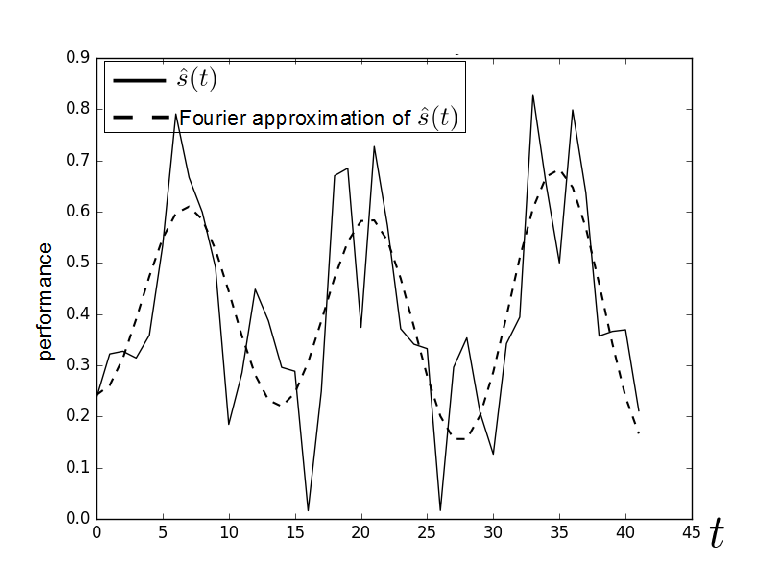
\includegraphics[width=10cm]{images/sample-fig.png}
    \caption{Contoh gambar.}
    \label{Fig: Contoh gambar}
\end{figure}

Contoh gambar terlihat pada Gambar \ref{fig:fig2}, \ref{fig:fig2a}, \ref{fig:fig2b}. Gambar diambil dari \cite{wibowo2016clustering}.

\begin{figure}[h]
    \centering
    \subfloat[]{
            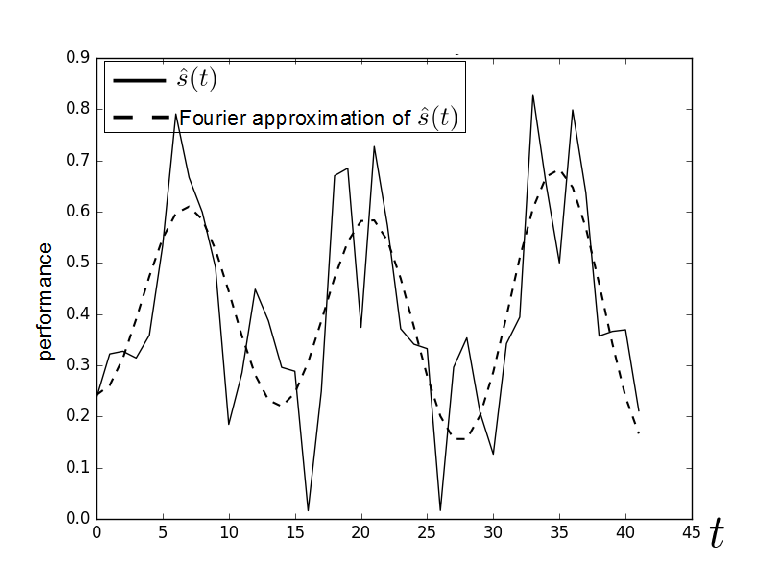
\includegraphics[width=0.45\textwidth]{images/sample-fig.png}
            \label{fig:fig2a}}
        % \hspace*{-1.2em}  % this is for giving horizontal space for fig 1 and fig 2.
    \subfloat[]{
            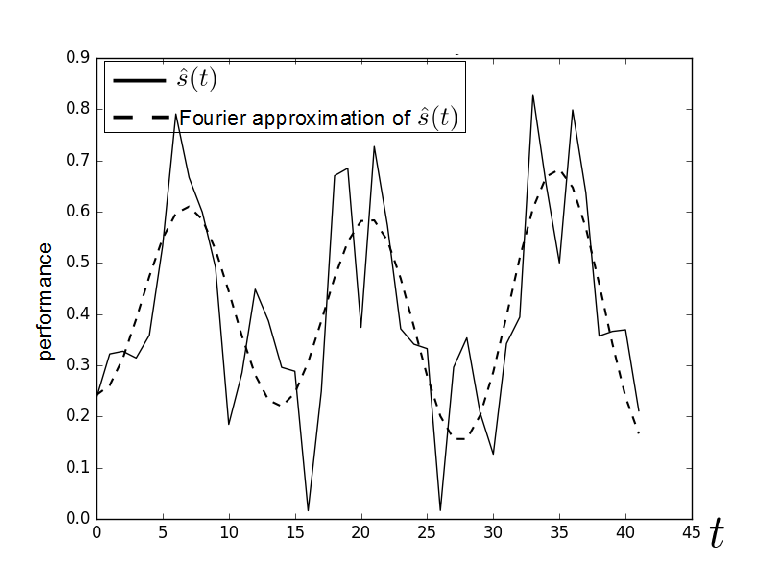
\includegraphics[width=0.45\textwidth]{images/sample-fig.png}
            \label{fig:fig2b}}
    \caption{(a) Figure 1 example and (b) Figure 2 example.}
    \label{fig:fig2}
\end{figure}

\section{Penulisan Tabel}

Contoh penulisan tabel bisa dilihat pada Tabel \ref{Tab: Tabel Tinggi Berat}.
\begin{table}[h]
    \caption{tabel ini}
    \centering
    \vspace{0em}  % adjust caption and table space as you like, default to no extra space
    \begin{tabular}{lrr}
        \hline
        ID & Tinggi Badan (cm) & Berat Badan (kg) \\
        \hline
        A23 & 173 & 62 \\
        A25 & 185 & 78 \\
        A10 & 162 & 70 \\ \hline
    \end{tabular}
    \label{Tab: Tabel Tinggi Berat}
\end{table}

Contoh penulisan tabel dengan nama kolom sangat panjang dengan bantuan \textit{tabulary} bisa dilihat pada Tabel \ref{Tab: Tabel Tinggi Berat Kolom Panjang}.

\begin{table}[h]
    \caption{tabel ini}
    \centering
    \vspace{0em}  % adjust caption and table space as you like, default to no extra space
    \begin{tabulary}{\linewidth}{lCC}
        \hline
        ID & Tinggi Badan Mahasiswa di Universitas Gadjah Mada (cm) & Berat Badan Mahasiswa di Universitas Gadjah Mada(kg) \\
        \hline
        A23 &  \multicolumn{1}{r}{173} &  \multicolumn{1}{r}{62} \\
        A25 &  \multicolumn{1}{r}{185} &  \multicolumn{1}{r}{78} \\
        A10 &  \multicolumn{1}{r}{162} &  \multicolumn{1}{r}{70} \\ \hline
    \end{tabulary}
    \label{Tab: Tabel Tinggi Berat Kolom Panjang}
\end{table}

Contoh penulisan tabel dengan gaya yang bersih bisa dilihat pada Tabel \ref{tab: Tabel Tinggi Berat Kolom Panjang Bersih}.

\begin{table}[h]
  \centering
  \caption{Tabel Tinggi Berat 2}
  \vspace{0em}  % adjust caption and table space as you like, default to no extra space
  \begin{tabulary}{\textwidth}{lRRRR}  % no vertical line if not needed
    \toprule
    & \multicolumn{2}{c}{Laki-laki} & \multicolumn{2}{c}{Perempuan} \\
    \cline{2-5}
    \multirow{-2}{*}{ID} & Tinggi Badan (cm) & Berat Badan (kg) & Tinggi Badan (cm) & Berat Badan (kg)\\
    \hline
    A23 \cite{lukito2016} & 173           & 62          & 173           & 62          \\
    A25                   & \textbf{185}  & 70          & \textbf{185}  & 70          \\
    A10                   & 162           & \textbf{78} & 162           & \textbf{78} \\
    \cline{2-5}
    Total & 520 & 210 & 520 & 210 \\
    \bottomrule
  \end{tabulary}
  \label{tab: Tabel Tinggi Berat Kolom Panjang Bersih}
\end{table}

\section{Penulisan formula}
Contoh penulisan formula
\begin{equation}
L_{\psi_z} = \{ t_i \mid v_z(t_i) \le \psi_z \}
\end{equation}

Contoh penulisan secara \textit{inline}: $\mathit{PV = nRT}$. Untuk kasus-kasus tertentu, kita membutuhkan perintah "mathit" dalam penulisan formula untuk menghindari adanya jeda saat penulisan formula.

Contoh formula \textbf{tanpa} menggunakan "mathit": $PVA = RTD$

Contoh formula \textbf{dengan} menggunakan "mathit": $\mathit{PVA = RTD}$

Untuk mengutip persamaan dapat juga menggunakan (\ref{eq:miqp-obj}). Persamaan dapat ditulis secara sentral pada file "equations/equations.tex".

    \inputeq{equations/equations}{miqp-obj}

\section{Contoh list}
Berikut contoh penggunaan list
\begin{enumerate}
    \item First item
    \item Second item
    \item Third item
\end{enumerate}

\section{Contoh \textit{highlight}}
Berikut contoh penggunaan \hly{\textit{highlight} kuning menggunakan} \verb|\hly{}|. Pengunaan \textit{highlight} tidak disarankan untuk dua paragraf sekaligus karena dapat mengakibatkan kerusakan dalam penomoran.

\hly{Gunakan perintah} \verb|\hly{}| yang terpisah untuk tiap paragrafnya seperti ini.

\hly{Penggunaan tanda \textit{curly bracket} \{ \} di dalam \textit{highlight} seperti penggunaan} \verb|\textit{}| \hlr{diperbolehkan, namun penghapusan otomatis oleh} \verb|"utilities/remove_highlight.ipynb"| \hly{tidak mendukung penghapusan \textit{nested bracket} seperti itu. Alternatifnya gunakan pemisahan} \textit{for the italic text} \hlg{seperti ini.}

\cleardoublepage \phantomsection
\chapter{Blok beda halaman}

\section{Membuat algoritma terpisah}

Untuk membuat algoritma terpisah seperti pada contoh berikut, kita dapat memanfaatkan perintah \textit{algstore} dan \textit{algrestore} yang terdapat pada paket \textit{algcompatible}. Pada dasarnya, kita membuat dua blok algoritma dimana blok pertama kita simpan menggunakan \textit{algstore} dan kemudian di-restore menggunakan \textit{algrestore} pada algoritma kedua. Perintah tersebut dimaksudkan agar terdapat kesinamungan antara kedua blok yang sejatinya adalah satu blok. 

\begin{algorithm}
    \caption{Contoh algorima}
    \label{findme}
    \begin{algorithmic} [1]
        \Procedure{CreateSet}{$v$}
        \State Create new set containing $v$
        \EndProcedure
        \algstore{myalg}
    \end{algorithmic}
\end{algorithm}

Pada blok algoritma kedua, tidak perlu ditambahkan caption dan label, karena sudah menjadi satu bagian dalam blok pertama. Pembagian algoritma menjadi dua bagian ini berguna jika kita ingin menjelaskan bagian-bagian dari sebuah algoritma, maupun untuk memisah algoritma panjang dalam beberapa halaman.

\begin{algorithm} 
    \begin{algorithmic} [1]
        \algrestore{myalg}
        \Procedure{ConcatSet}{$v$}
        \State Create new set containing $v$
        \EndProcedure
    \end{algorithmic}
\end{algorithm}

\newpage  % used to simulate change page, delete this for usage
\section{Membuat tabel terpisah}

Untuk membuat tabel panjang yang melebihi satu halaman, kita dapat mengganti kombinasi \textit{table + tabular} menjadi \textit{longtable} dengan contoh sebagai berikut.

\begin{longtable}{| c | c |} 
    \caption{Contoh tabel panjang}
    \label{tab:myfirstlongtable} \\
    \hline
    header 1 & header 2 \\
    \hline \hline
    foo & bar \\ \hline 
    foo & bar \\ \hline
    foo & bar \\ \hline
    foo & bar \\ \hline
    foo & bar \\ \hline
    \newpage  % used to simulate change page, delete this for usage
    foo & bar \\ \hline
    foo & bar \\ \hline
    foo & bar \\ \hline
    foo & bar \\ \hline
    foo & bar \\ \hline
    foo & bar \\ \hline
\end{longtable}

\begin{longtable}{ccc}
    \caption{My clean table with continue message}
    \label{tab:cleanlongtable} \\
    \hline
    Column 1 & Column 2 & Column 3\\\hline
    \endfirsthead
    \multicolumn{3}{@{}l}{\ldots continued}\\\hline
    Column 1 & Column 2 & Column 3\\\hline
    \endhead % all the lines above this will be repeated on every page
    \hline
    \multicolumn{3}{r@{}}{continued \ldots}\\
    \endfoot
    \hline
    \endlastfoot
    A & B & C\\     A & B & C\\
    A & B & C\\     A & B & C\\
    A & B & C\\     A & B & C\\
    \newpage  % used to simulate change page, delete this for usage
    A & B & C\\     A & B & C\\
    A & B & C\\     A & B & C\\
    A & B & C\\     A & B & C\\
    A & B & C\\     A & B & C\\
\end{longtable}

% NOTE: kelemahan dari penggunaan longtable adalah ketidakmampuannya untuk dikombinasikan dengan \begin{table}[t] maupun \begin{table}[h], di mana penggunaan \begin{table}[t] atau \begin{table}[h] akan menghilangkan kemampuan longtable itu sendiri untuk dapat berada pada dua halaman. 
    
Kombinasi dari \verb|\tabulary| yang mendukung \textit{auto-wrap} dengan \verb|\longtable| yang mendukung tabel antar halaman adalah fungsi yang disediakan \texttt{thesisdtetiugm} yaitu \verb|\ltabulary|.

\begin{ltabulary}{LLL}
    % firsthead start for header of table on first appearance
    \toprule
    Column 1 & Column 2 & Column 3 with very very very very very very very long column name\\\midrule
    \endfirsthead
    % newpage head, just copy paste after continued message
    \multicolumn{3}{@{}l}{\ldots continued}\\\toprule  % continued message, change the number with number of columns
    Column 1 & Column 2 & Column 3 with very very very very very very very long column name\\\midrule
    \endhead % all the lines between \endfirsthead and \endhead will be used on the next page
    % every foot use continued from \endhead to \endfoot
    \bottomrule
    \multicolumn{3}{r@{}}{continued \ldots}\\
    \endfoot
    % every foot will only use \bottomrule from \endfoot to \endlastfoot
    \bottomrule
    \endlastfoot
    x&y&z\\
    x&y&z\\
    x&y&z\\
    x&y&z\\
    x&y&z\\
    x&y&z\\
    x&y&z\\
    x&y&z\\
    x&y&z\\
    x&y&z\\
    x&y&z\\
    x&y&z\\
    x&y&z\\
    x&y&z\\
    x&y&z\\
    x&y&z\\
    x&y&z\\
    x&y&z\\
    x&y&z\\
    x&y&z\\
    x&y&z\\
    x&y&z\\
    x&y&z\\
    x&y&z\\
    x&y&z\\
\end{ltabulary}

\section{Menulis formula terpisah halaman}

Terkadang kita butuh untuk menuliskan rangkaian formula dalam jumlah besar sehingga melewati batas satu halaman. Solusi yang digunakan bisa saja dengan memindahkan satu blok formula tersebut pada halaman yang baru atau memisah rangkaian formula menjadi dua bagian untuk masing-masing halaman. Cara yang pertama mungkin akan menghasilkan alur yang berbeda karena ruang kosong pada halaman pertama akan diisi oleh teks selanjutnya. Sehingga di sini kita dapat memanfaatkan \textit{align} yang sudah diatur dengan mode \textit{allowdisplaybreaks}. Penggunakan \textit{align} ini memungkinkan satu rangkaian formula terpisah berbeda halaman. 

Contoh sederhana dapat digambarkan sebagai berikut.

\begin{align*}
x &= y^2\\
x &= y^3\\
a + b &= c\\
x &= y - 2\\
a + b &= d + e \tag{\stepcounter{equation}\theequation}\\
x^2 + 3 &= y\\
a(x) &= 2x\\
b_i &= 5x\\
10x^2 &= 9x\\
2x^2 + 3x + 2 &= 0\\
5x - 2 &= 0\\
d &= \log x\\
y &= \sin x
\end{align*}

\section{Memasukkan program yang panjang}

Untuk memasukkan program yang panjang, kita menggunakan bantuan dari \verb|\lstinputlisting|. Karena \verb|\lstinputlisting| melakukan impor satu file secara utuh, sangat dianjurkan untuk menulis satu fungsi spesifik per file.

\lstinputlisting[%
    language=Python,%
    caption={Potongan \textit{code} berbahasa Python.},%
    label={lst:sample_code_py}]%
    {codes/sample-code.py}

\cleardoublepage \phantomsection
\chapter{<<Chapter name>>}



\cleardoublepage \phantomsection
\chapter{<<Chapter name>>}
\cleardoublepage \phantomsection
\chapter{<<Chapter name>>}


%======================================

%======================================
%  References
%======================================
\cleardoublepage \phantomsection
\thereferences
\bibliographystyle{bibtex/IEEEtran}
\bibliography{bibtex/references}
%======================================

%======================================
%  Appendix
%======================================
\cleardoublepage \phantomsection
\chapterappendix{contents/appendix/appendix}
%======================================

\end{document}